\documentclass[border=5pt]{standalone}
\usepackage{tikz}
\usetikzlibrary{positioning,arrows.meta,calc}
\usepackage{xcolor}

\definecolor{framecol}{RGB}{69,90,120}
\definecolor{okcol}{RGB}{52,168,83}
\definecolor{failcol}{RGB}{234,67,53}
\definecolor{tlcol}{RGB}{120,120,140}

\begin{document}
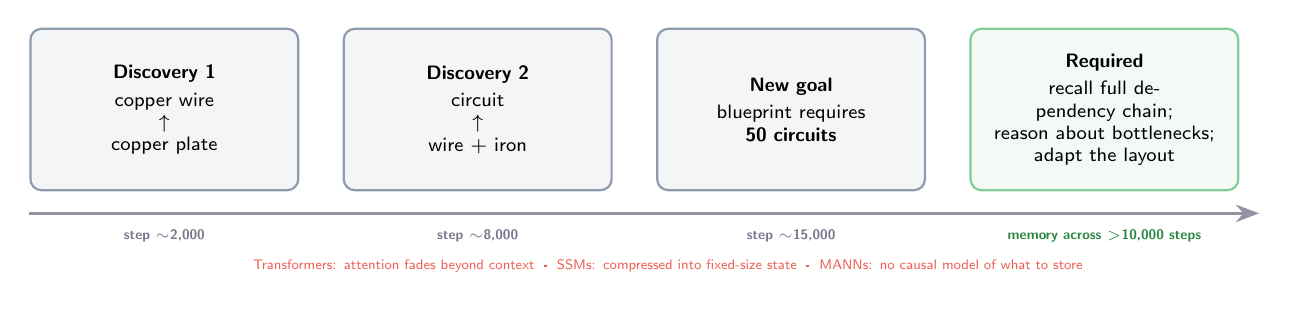
\begin{tikzpicture}[
    font=\sffamily,
    frame/.style={draw=#1!60, fill=#1!6, rounded corners=4pt, thick,
                  minimum height=2.05cm, text width=3.05cm, align=center,
                  font=\scriptsize\sffamily, inner sep=5pt},
    steplab/.style={font=\tiny\sffamily\bfseries, color=tlcol},
    tl/.style={->, >=Stealth, very thick, color=tlcol!80},
]

% ---- Frames ----
\node[frame=framecol] (f1) {
  \textbf{Discovery 1}\\[2pt]
  copper wire\\$\uparrow$\\copper plate
};
\node[frame=framecol, right=0.55cm of f1] (f2) {
  \textbf{Discovery 2}\\[2pt]
  circuit\\$\uparrow$\\wire $+$ iron
};
\node[frame=framecol, right=0.55cm of f2] (f3) {
  \textbf{New goal}\\[2pt]
  blueprint requires\\\textbf{50 circuits}
};
\node[frame=okcol, right=0.55cm of f3] (f4) {
  \textbf{Required}\\[2pt]
  recall full dependency chain;\\
  reason about bottlenecks;\\
  adapt the layout
};

% ---- Timeline ----
\draw[tl] ($(f1.south west)+(0,-0.28)$) -- ($(f4.south east)+(0.25,-0.28)$);
\node[steplab, anchor=north] at ($(f1.south)+(0,-0.36)$) {step $\sim$2{,}000};
\node[steplab, anchor=north] at ($(f2.south)+(0,-0.36)$) {step $\sim$8{,}000};
\node[steplab, anchor=north] at ($(f3.south)+(0,-0.36)$) {step $\sim$15{,}000};
\node[steplab, anchor=north, color=okcol!80!black] at ($(f4.south)+(0,-0.36)$) {memory across $>$10{,}000 steps};

% ---- Failure annotations under timeline ----
\node[font=\tiny\sffamily, color=failcol!85, anchor=north, text width=13.9cm, align=center]
  at ($(f2.south east)+(0.7,-0.75)$) {
  Transformers: attention fades beyond context \;·\; SSMs: compressed into fixed-size state \;·\; MANNs: no causal model of what to store
};

\end{tikzpicture}
\end{document}
